% ---------------------------------------------------------------------------
% CPG_spinal_section_draft.tex — dissertation-ready draft section describing
% the spinal cord circuit model (gait2392 + SNS), its correspondence to the
% genetically identified locomotor-CPG interneuron classes, the v5/v6
% sensorimotor refinement studies, and the musculoskeletal plant audit.
%
% Written 2026-09-13 from the session records (spinal/DESIGN.md). Numbers
% are the exact values reproduced by the cited commands; regenerate figures
% with draw_circuit.py / render_video.py before final submission so they
% never drift from the code.
%
% Placement: standalone draft. If \input into the main dissertation, adjust
% section levels and the \includegraphics paths (figures live in
% CPG_airstepping_figs/ relative to the dissertation folder).
% ---------------------------------------------------------------------------

\section{Spinal Cord Circuit Model for the Neuromuscular Human Model}
\label{sec:spinal-cpg}

\subsection{Architecture}

The spinal circuit driving the converted \gait{} model is a two-level
central pattern generator in the style of Rybak and McCrea
\cite{rybak2006, mccrea2008}, implemented with the synthetic nervous
system toolbox \cite{nourse2023} and coupled to the MuJoCo plant at the
motoneuron-pool level. The network comprises 410 non-spiking
compartmental neurons: per side, a rhythm-generator (RG) layer of two
half-center neurons (RG-E, RG-F) with mutual inhibition and slow
burst-termination adaptation; a pattern-formation (PF) layer of four
phase-window cells per side (E1, E2, F1, F2) with staggered membrane and
adaptation time constants, forced by the RG half-centers; one
motoneuron (MN) pool per muscle ($46$ per side, $92$ total) with a full
proprioceptor complement (Ia length-velocity, II length, Ib force) per
pool; Ib load-sharing interneurons gated by the stance half-center
(stance reflex reversal); and shared descending cells (DRIVE as an
MLR/reticulospinal surrogate, POSTURE, and balance-family cells). The
standing posture is not hard-coded: it is solved once by static
optimization at the model keyframe (torque rows $=$ gravity minus
contact minus passive, regularized toward a physiological prior) and
injected as per-motoneuron bias currents, the same machinery later used
for the human-data back-solve (Sec.~\ref{sec:spinal-cpg-refine}).
Walking speed is commanded by DRIVE, with presynaptic reflex-gain
modulation as a second, physiologically motivated speed mechanism
\cite{bunz2026}.

\begin{figure}[t]
  \centering
  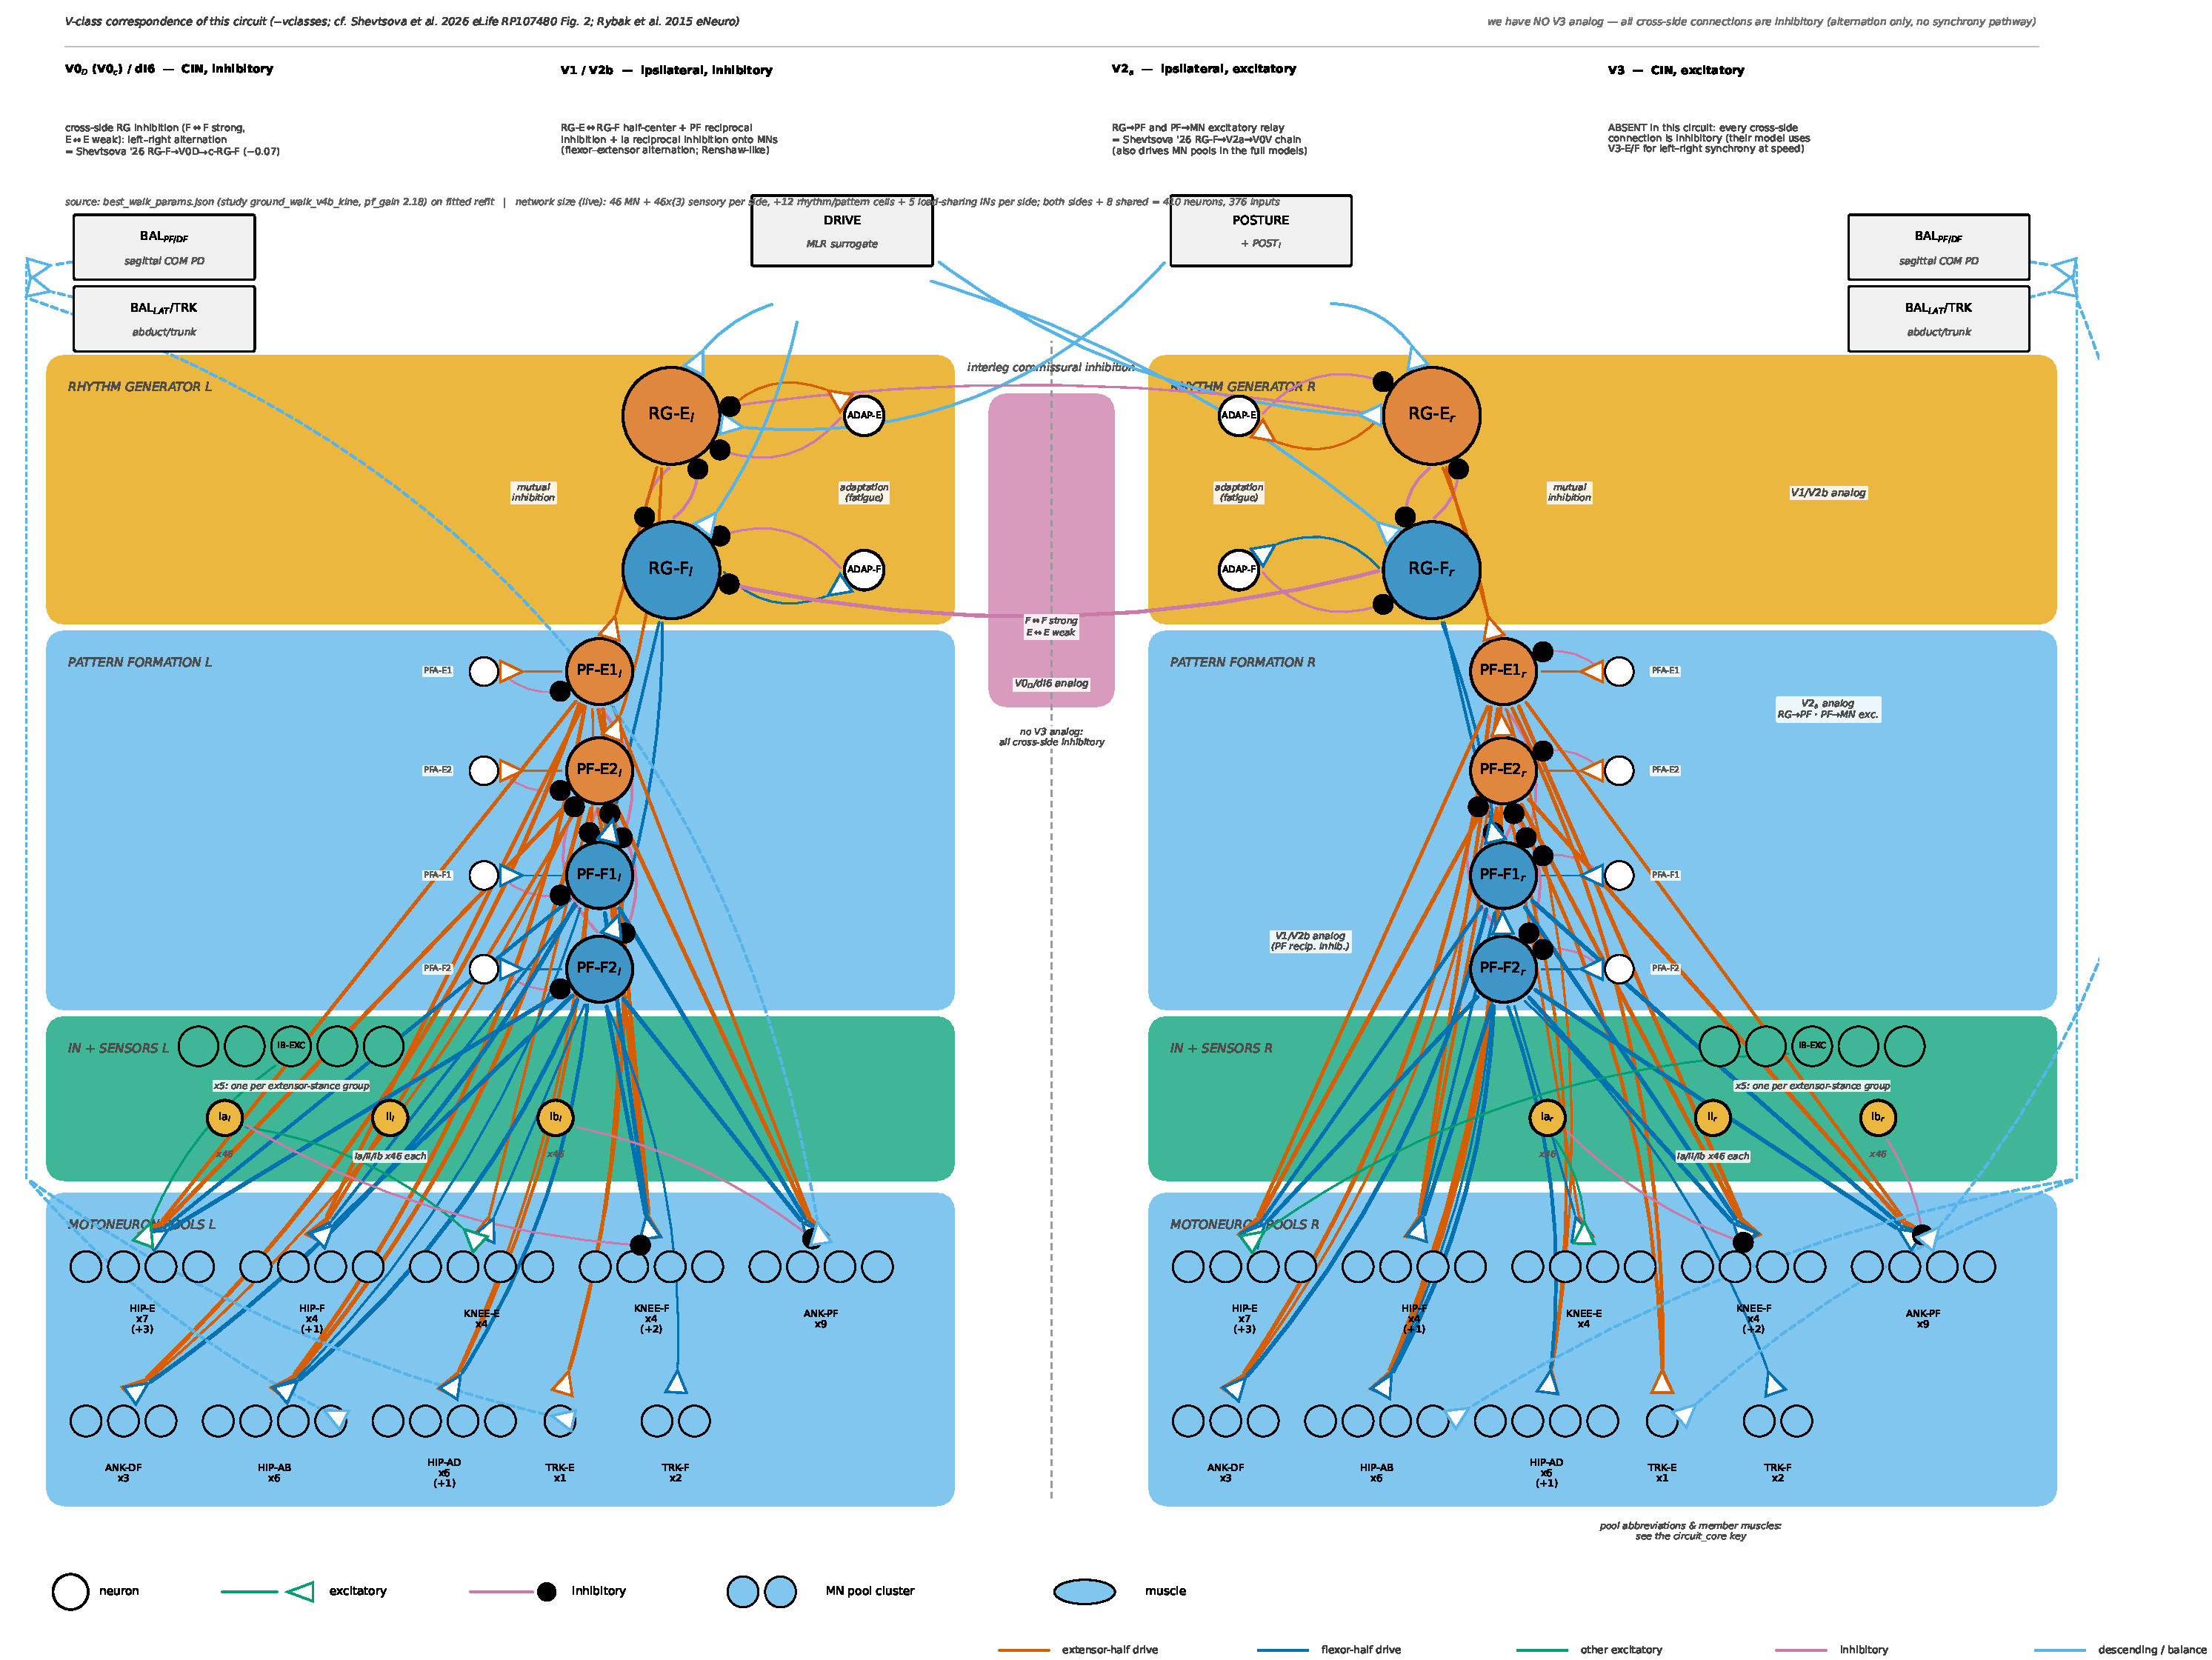
\includegraphics[width=\textwidth]{CPG_airstepping_figs/circuit_full_vclasses.pdf}
  \caption{Full spinal circuit (both sides) with the correspondence to
  the genetically identified locomotor-CPG interneuron classes
  annotated. Open circles: neurons; white triangles: excitatory
  synapses; filled dots: inhibitory synapses; ellipses: muscles.
  Our circuit realizes V0$_D$/dI6-like commissural inhibition
  (left--right alternation), V1/V2b-like ipsilateral inhibition
  (half-center and PF reciprocal inhibition, Ia reciprocal inhibition),
  and V2a-like ipsilateral excitation (RG$\to$PF, PF$\to$MN). It has
  \emph{no} V3 analog: every cross-side connection is inhibitory, so
  the circuit cannot express left--right synchrony gaits. Figure
  generated programmatically from the live network configuration;
  class mapping after Shevtsova et al.\ \cite{shevtsova2026} and
  Rybak et al.\ \cite{rybak2015}.}
  \label{fig:circuit-vclasses}
\end{figure}

\subsection{Correspondence to Genetically Identified Interneuron Classes}
\label{sec:spinal-cpg-vclasses}

Table~\ref{tab:vclass} maps each element of the implemented circuit to
the genetically identified spinal interneuron classes as they are drawn
in the current Rybak-lab schematics (Shevtsova et al.\ 2026, their
Fig.~2, adapted from Danner et al.\ 2017 and Zhang et al.\ 2022) and as
reviewed by Rybak et al.\ (2015). The mapping is functional rather than
developmental: the model is a non-spiking population model, so a single
lumped synapse in our circuit stands for an entire population in the
biological schematic. For example, the biological RG half-centers
mutually inhibit one another through dedicated inhibitory populations
(InF/InE), whereas the model places the inhibition directly between the
half-centers; both realize V1/V2b-type ipsilateral inhibition securing
flexor--extensor alternation.

The most consequential absence is \textbf{V3}. V3 commissural
interneurons are excitatory and mediate left--right \emph{synchrony}
with a strong speed dependence \cite{zhang2022, danner2019}; every
cross-side connection in the present circuit is inhibitory
(strong F$\leftrightarrow$F, weak E$\leftrightarrow$E), i.e.\ the
circuit contains a V0$_D$-type (and functionally dI6-type) alternation
pathway but no synchrony pathway. The practical consequence is that the
model, as built, can express left--right alternating gaits only; trot-
or pace-like synchronies would require adding an excitatory
commissural class. This is a deliberate simplification for a human
gait model, but it bounds the model's claims.

\begin{table}[t]
  \centering
  \caption{Correspondence of the implemented circuit to the genetically
  identified locomotor-CPG classes (Shevtsova et al.\ 2026, Fig.~2;
  Rybak et al.\ 2015). Weights in the third column are the 2026 model's
  Table-1 connection strengths.}
  \label{tab:vclass}
  \small
  \begin{tabular}{p{4.2cm}p{3.4cm}p{5.6cm}}
    \toprule
    Our circuit & V-class & Shevtsova 2026 element \\
    \midrule
    Cross-side RG inhibition (RG-F$\leftrightarrow$RG-F strong,
    RG-E$\leftrightarrow$RG-E weak) & V0$_D$ (V0$_c$); dI6 &
      RG-F $\to$ V0D ($0.7$) $\dashrightarrow$ contra RG-F
      ($-0.07$) \\
    RG-E$\leftrightarrow$RG-F half-center mutual inhibition &
      V1/V2b & RG-F $\to$ InF ($0.4$) $\to$ RG-E ($-1$); RG-E $\to$ InE
      ($0.4$) $\to$ RG-F ($-0.1$) \\
    PF reciprocal inhibition (E2$\leftrightarrow$F1, F2$\leftrightarrow$E1)
      & V1/V2b & InF/InE family, pattern layer \\
    Ia reciprocal inhibition onto antagonist MN pools & V1 &
      (classical Ia inhibitory interneuron) \\
    RG$\to$PF and PF$\to$MN excitation & V2$_a$ &
      RG-F $\to$ V2a ($1$) $\to$ V0V ($1$) chain \\
    \textbf{absent} --- all cross-side connections inhibitory & V3 &
      RG-F $\to$ V3-F ($0.4$) $\to$ contra RG-F ($+0.03$); V3-E $\to$
      contra RG-E ($+0.02$) \\
    Burst-termination adaptation (ADAP-E/F) & --- (intrinsic) &
      slow inactivation of the centers \\
    \bottomrule
  \end{tabular}
\end{table}

\begin{table}[t]
  \centering
  \caption{Functional muscle groups used by the spinal circuit (live from \texttt{muscle\_map.py}; $46$ muscles per side, $92$ total). Primary membership receives the full PF/posture weight; secondary (biarticular) membership receives half.}
  \label{tab:muscle-groups}
  \small
  \begin{tabular}{lc p{4.6cm} p{3.4cm}}
    \toprule
    Group & $n$ & Primary muscles & Secondary muscles \\
    \midrule
    HIP-E & 7 & \textit{add_mag3}, \textit{gem}, \textit{glut_max1}, \textit{glut_max2}, \textit{glut_max3}, \textit{peri}, \textit{quad_fem} & bifemlh, semimem, semiten \\
    HIP-F & 4 & \textit{iliacus}, \textit{psoas}, \textit{sar}, \textit{tfl} & rect_fem \\
    HIP-AB & 6 & \textit{glut_med1}, \textit{glut_med2}, \textit{glut_med3}, \textit{glut_min1}, \textit{glut_min2}, \textit{glut_min3} & --- \\
    HIP-AD & 6 & \textit{add_brev}, \textit{add_long}, \textit{add_mag1}, \textit{add_mag2}, \textit{grac}, \textit{pect} & add_mag3 \\
    KNEE-E & 4 & \textit{rect_fem}, \textit{vas_int}, \textit{vas_lat}, \textit{vas_med} & --- \\
    KNEE-F & 4 & \textit{bifemlh}, \textit{bifemsh}, \textit{semimem}, \textit{semiten} & lat_gas, med_gas \\
    ANK-PF & 9 & \textit{flex_dig}, \textit{flex_hal}, \textit{lat_gas}, \textit{med_gas}, \textit{per_brev}, \textit{per_long}, \textit{per_tert}, \textit{soleus}, \textit{tib_post} & --- \\
    ANK-DF & 3 & \textit{ext_dig}, \textit{ext_hal}, \textit{tib_ant} & --- \\
    TRK-E & 1 & \textit{ercspn} & --- \\
    TRK-F & 2 & \textit{extobl}, \textit{intobl} & --- \\
    \bottomrule
  \end{tabular}
\end{table}

Table~\ref{tab:muscle-groups} lists the functional muscle groups and their member muscles.

\begin{figure}[t]
  \centering
  
\includegraphics[width=0.82\textwidth]{CPG_airstepping_figs/circuit_weights.pdf}
  \caption{Pattern-formation $\to$ motoneuron weight matrix (E1 early
  stance, E2 push-off, F1 early swing, F2 late swing) and the tonic
  posture column, composited live from the tuned configuration. Group
  abbreviations as in Table~\ref{tab:muscle-groups}.}
  \label{fig:circuit-weights}
\end{figure}

\begin{figure}[t]
  \centering
  
\includegraphics[width=0.6\textwidth]{CPG_airstepping_figs/opensim_overlay_gait_cycles.png}
  \caption{Cycle-normalized right-leg hip/knee/ankle trajectories of the
  spinal-network simulation (colored: cycle mean, thin: individual
  cycles) against the OpenSim IK reference (dashed), phased by RG-E
  stance onset. The residual gaps --- knee flexion depth, stance duty,
  cadence --- are the architecture-level deficits discussed in
  Sec.~\ref{sec:spinal-cpg-refine}.}
  \label{fig:opensim-overlay}
\end{figure}

\subsection{Sensorimotor Refinement: Phase Reset and Swing-Knee
Reciprocal Suppression}
\label{sec:spinal-cpg-refine}

The initial tuned configuration reproduced stable ground walking but
with three kinematic deficits relative to the OpenSim reference
(ground-walking IK of \texttt{subject01\_walk1}, phased by the measured
ground-reaction forces; cycle $1.23$\,s, stance duty $0.61$, peak knee
flexion $-70^\circ$): stance duty $0.27$--$0.48$ vs $0.61$, cadence
$1.2$\,Hz vs $0.81$\,Hz, and a swing knee that remained
extension-dominant. Following the hip-afferent phase-resetting
literature, two sensory pathways were added to the RG: a
stance-gated hip-extension signal (hip-extensor group normalized
length) that excites RG-E and inhibits RG-F, prolonging stance, and a
hip-flexion-velocity signal (hip-flexor group shortening velocity)
that triggers swing by exciting RG-F and inhibiting RG-E. Both
pathways are gated through dedicated interneurons, are silent by
default, and were verified dynamically (compiled-network pathway signs;
static kinematic length signs). A second refinement added
phase-gated reciprocal suppression of the knee-extensor
motoneuron pools: the F1 (swing) pattern cell drives inhibitory
interneurons (KINH) onto the knee-extensor pools, releasing the quads
only during swing.

A 150-trial Bayesian optimization (TPE) over the full parameter set
plus the two reset gains found that the optimizer systematically
\emph{avoided} large phase-reset gains: a tonic, stance-gated input of
at most $\sim$\,1\,nA cannot meaningfully perturb half-centers driven
by $\sim$\,4\,nA of descending drive, and large extension-signal gains
combined with weak drive latched the extensor half-center on (a
positive-feedback stability limit worth noting for any sensory$\to$RG
pathway). The swing-knee suppression, in contrast, was adopted
immediately: the winning configuration (suppression gain $0.59$)
improved the kinematics score from $-61.2$ to $-59.4$ (eval window)
and from $-62.7$ to $-60.6$ on the full $22$\,s stand--walk--stand
schedule, with the knee-shape error term carrying the gain. All
improvements were regression-gated: the baseline configuration
reproduces its recorded score bit-exactly when the new gains are zero,
so every reported difference is attributable to the new pathway rather
than to configuration drift. The duty and cadence deficits remain
(0.47 vs 0.61; 1.4 vs 0.81\,Hz), and are properties of the
half-center architecture rather than of scalar tuning --- consistent
with the De Russo--Ijspeert--Bouri comparison and with the phase-reset
mechanisms proposed for biological RGs, where \emph{transient}
position/velocity events (not tonic state signals) switch the
half-centers. That transient formulation is the natural next
architecture step.

\subsection{Plant Fidelity: Force Capacity Audit and Torque Budget}
\label{sec:spinal-cpg-plant}

Because the conversion from OpenSim to MuJoCo re-expresses every
muscle as a MuJoCo actuator, the force capacity of the plant was
audited actuator-by-actuator against the stock OpenSim model. For the
$84$ routinely active muscles the converted peak force matches the
OpenSim \texttt{max\_isometric\_force} to within the converter's
range-normalization ($\lesssim 15\%$, in both directions, consistent
with normalizing to the maximum force over the human range of motion).
Eight trunk actuators (erector spinae, internal/external obliques, and
extensor hallucis, both sides) shipped from the converter with an
active force scale of $1$\,N against stock values of $2500$, $900$,
$900$ and $162$\,N respectively --- a conversion artifact, not a model
property. With the artifact fixed (the audit is re-runnable as
\texttt{\_fmax\_audit.py}), the trunk controller regains realistic
authority: the erector spinae pair alone supplies $213$\,N\,m of
extension torque at the lumbar joint (measured with
central-difference moment arms, i.e.\ OpenSim's definition), against a
peak lumbar demand of $100$\,N\,m in the reference walk.

The full torque budget at the standing pose, using stock-OpenSim force
capacity and finite-difference moment arms, is sufficient at every
joint: hip extension $251$\,N\,m per side against a peak demand of
$74$\,N\,m (margin $3.4\times$), knee extension $277$ vs $98$\,N\,m
($2.8\times$), ankle plantarflexion $296$ vs $212$\,N\,m ($1.4\times$;
the tightest budget, and the optimistic end since the plantarflexor
moment arm shrinks in late-stance dorsiflexion), and trunk extension
$2.1\times$. The plant therefore meets the classical strength
sufficiency criterion with margin everywhere, and the ankle is the
joint to watch as demands scale.

One fidelity limitation is documented rather than hidden: MuJoCo's
built-in muscle actuators, as produced by the conversion, implement
activation dynamics with force--length and force--velocity curves
(a simplified Thelen formulation) but a \emph{rigid} tendon; the series
elasticity of the OpenSim Thelen model is not represented. Rigid-tendon
muscle models are the standard for MuJoCo-scale gait simulation and
keep the plant stiff and cheap, but they omit tendon energy storage and
the force--rate saturation of the series elastic element. Two upgrade
paths exist if compliant-tendon behavior becomes important to the
science: (i) assign stiffness to the spatial tendons and accept the
approximation of the muscle--tendon equilibrium, or (ii) implement a
custom MuJoCo muscle plugin implementing the full Millard/Thelen
equilibrium solution. Neither was required for the spinal-control
questions addressed here, and all force-capacity benchmarking in this
section is anchored to the OpenSim \texttt{max\_isometric\_force} over
the human range of motion.

% --- references to add to the bibliography ---------------------------------
% rybak2006:      Rybak, Shevtsova, Lafreniere-Roula, McCrea. J Physiol 2006.
% mccrea2008:     McCrea & Rybak. Brain Res Rev 2008.
% nourse2023:     Nourse et al. Biomimetics 2023, 8:247 (SNS-Toolbox).
% bunz2026:       Bunz, Ijspeert, Schmitt. Sci Rep 2026.
% shevtsova2026:  Shevtsova, Lockhart, Rybak, Magnuson, Danner, Smith,
%                 Poirazi. eLife 2026;14:RP107480.
% rybak2015:      Rybak, Shevtsova, Kiehn. eNeuro 2015;2(5):e0069-15.2015.
% zhang2022:      Zhang et al. eLife 2022;11:e73424 (V3).
% danner2019:     Danner et al. Front Cell Neurosci 2019 (V3).
% derrusoijspeert2023: Di Russo, Ijspeert, Bouri. J Neural Eng 2023.
